\documentclass[11pt,a4paper]{article}
\usepackage[latin1]{inputenc}
\usepackage{amsmath}
\usepackage{amsfonts}
\usepackage{mathtools}
\usepackage{array}
\usepackage{pifont}
\usepackage{ifsym}
\usepackage{booktabs}
\usepackage{listings}
\usepackage{amssymb}
\usepackage{graphicx}
\usepackage{longtable}
\usepackage{tabularx}
\usepackage{enumitem}
\usepackage{url}
\usepackage[margin=0.8in]{geometry}
\usepackage[toc,page]{appendix}
\usepackage{etoolbox}
\usepackage{morefloats}
\usepackage{multirow}
\usepackage[hidelinks]{hyperref}
\usepackage{float} % Allows putting an [H] in \begin{figure} to specify the exact location of the figure
\usepackage{verbatim}
\usepackage{listings}
\usepackage[usenames,dvipsnames]{color}

\usepackage{fullpage}

\graphicspath{{img/}}

\patchcmd{\thebibliography}{\section*}{\subsection}{}{}

\newcolumntype{C}[1]{>{\centering\let\newline\\\arraybackslash\hspace{0pt}}m{#1}}

% Table padding
\renewcommand{\arraystretch}{1.5}

\begin{document}

\begin{titlepage}

\begin{center}

\includegraphics[width=0.5\textwidth]{img/University_Logo}\\

\textsc{\LARGE Swansea University }\\[0.5cm]
\textsc{\large MEng Computing }\\[2cm]

{ \huge \bfseries Group Project CS-M04}\\[0.2cm]
\textsc{\large Team Structure, Methodology, Requirements and Specifications}\\[1.5cm]

\begin{minipage}{0.4\textwidth}
\begin{flushleft}

\emph{Authors:}\\
Adam \textsc{Barrell} {\scriptsize \emph{(632975)}} \\
Thomas \textsc{Milner} {\scriptsize \emph{(637755)}} \\
Lewis \textsc{Hancock} {\scriptsize \emph{(xxxxxx)}} \\
Christopher \textsc{Lewis} {\scriptsize \emph{(xxxxxx)}} \\

\end{flushleft}
\end{minipage}
\begin{minipage}{0.4\textwidth}
\begin{flushright}

\emph{Supervisor:}\\
Parisa \textsc{Eslambolchilar}

\end{flushright}
\end{minipage}\\[1.3cm]

{\today}
\end{center}

\end{titlepage}

\newpage 
\setcounter{page}{1}
\pagenumbering{roman}
\tableofcontents

\newpage
\setcounter{page}{1}
\pagenumbering{arabic}
\section{Introduction}
This document, White Rock Digital Trails: Interim Document, shall guide the reader through the current state of the project. This includes the design of user interfaces, implementation of features and project management tasks such as a schedule update and analysis of any risks the project has encountered.
\subsection{Purpose}
The document aims to inform the reader of all progress made on the project since the last document. It was originally created as part of an MEng Computing degree at Swansea University, under the supervision of Parisa Eslambolchilar, for the White Rock team (TODO:CITE). The document is also suitable for third parties interested in the development of White Rock Digital Trails, subject to permission from the authors. The document acts a follow-up document to the previously written Milestone 1: (TODO: find name and cite).
\subsection{Overview}
%- Outline of Document (what we cover in the document).

\section{Technology Choices}
\subsection{Android}
As the project includes an Android application, it has been important to choose effective software and technology for development, this ranges from the Integrated Development Environment (IDE) used by the development team to the hardware devices used for testing.

\subsubsection{IDE}
There were three potential IDE choices for Android development, Eclipse, Android Studio and NVIDIA Nsight Tegra, a Visual Studio plugin for Android.

For this project the choice was straightforward, the team has experience with Android and it has been around the longest, providing a stable and familiar programming environment helping keep efficiency levels high. Whilst Android Studio is now the supported IDE by Google, it is still relatively new software and offers a big change compared to Eclipse. NVIDIA Nsight Tegra, whilst a powerful IDE, would have provided a drastic change in environment for developers without Visual Studio familiarity. It is also more likely to take valuable development hours away to configure for every developer.

\subsubsection{Devices}
A number of devices are being used during development of the application. They range in size, power and operating system to ensure that we have a reasonable set of possible configurations to test our application.

\begin{longtable}{|c|p{8cm}|}\hline
\textbf{Device} & \textbf{Specification} \\ \hline
Tesco Hudl & \begin{itemize}
\item 7 Inch IPS LCD.
\item 1440 x 900 Resolution.
\item 10-point multi-touch screen.
\item 1.5GHz A9 Quad-core processor.
\item 1GB RAM.
\item Mali 400 Quad-core GPU.
\item Dual-band Wi-Fi.
\item Bluetooth 4.0.
\item GPS.
\end{itemize} \\ \hline
Other Device & spec \\ \hline
Other Device 2 & spec \\ \hline

\end{longtable}

\subsubsection{Minimum Supported OS}
To ensure the widest user base possible can access the application, the application will support Android devices running on Android 2.3 or higher. This is over 90\% of all Android phones https://developer.android.com/about/dashboards/index.html TODO: ADD TO BIB.

\subsection{The API}
\label{sec:techAPI}
To keep the Application and the website in sync, and allow for future developments such as additional applications, an RESTful API (Application Programming Interface) was created.

\begin{description}
\item[API] Application Programming Interface, In general an API is a method of interaction between two software components through code. This often take the form of a Library, although a web API generally takes the form of several remote calls which are exposed to the user of the API. 

\item[REST] Representational State Transfer, is a architecture style which was used to design HTTP/1.1 (Hyper Text Transfer Protocol Version 1.1) and the URI (Universal Resource Identifier) standards. It consists of a set of constraints on components, data and there connections. The primary constraint is a Client-Sever separation, with the server being responsible for data storage, and the client responsible for the user interface and user state. The server is also required to be stateless which means no client context can be stored on the server.
\end{description}

For the API the Slim Framework\cite{slim} was chosen. This framework is designed for creating lightweight restful API's and websites and provides a versatile and well tested bases for the work. There were several other choices for this framework, but Slim was chosen because it was the most popular and well documented option. The Paris ORM(Object Relation Mapper) Framework\cite{paris} was also chosen to assist in database access. The ORM uses simple database models to reduce the steps in the process of interacting with the database. This framework makes it very easy to work with databases, drastically cutting the code needed to retrieve data and process it into objects. Paris was the only ORM of this type we could find for PHP and  For example, if you had a simple database with just Documents and Users it would be possible to model this using just the code below, in Listing~\ref{lst:model}. There are two model definitions and then 2 very basic lines of code which return a user object in the variable \lstinline{$user}. The second line then queries \lstinline{$user} to get all the documents associated with that user~\cite{TomMilestone2}. 

\begin{lstlisting}[captionpos=b, caption=Model Snippet, label=lst:model, frame=single]
class User extends Model {
	public function documents(){
		return $this->has_many('Document');
	}
}

class Document extends Model{
	public function user(){
		return $this->belongs_to('User');
	}
}

$user = Model::factory('User')->find_one($id); 
$documents = $user->documents()->find_many();
\end{lstlisting}

\subsection{The Server}
The project is currently hosted on an Amazon EC2 server owned by a group member. Having a private server like this has allowed us to configure it as we require. The server is currently running Ubuntu Linux Server Edition with Apache Webserver, PHP and MySQL database installed. Git is used to push documents up to the server which are then automatically copied into the correct folder for the webserver. Each part of the project can then be given a unique subdomain for testing purposes. Currently the API is hosted at \url{http://whiterockapi.tmilner.co.uk/} and the Web Portal is at \url{http://whiterock.tmilner.co.uk}.

\begin{description}
\item[Ubuntu Linux Server Edition] An open source operating system based upon the Linux kernel. Free to use and modify, and developed specifically for use of servers. 

\item[Apache Webserver] An highly popular open source web server. Free to use and installed as default in Ubuntu Linux Server Edition.

\item[PHP] The programming language that is being used to develop the web service. It requires a runtime which is installed as an addon to Apache Webserver. 

\item[MySQL] A popular SQL (Structured Query Language) database system. Developed by Sun Enterprises and free to use. 

\item[Git] A distributed source control system. Used to track changed to code and share changed between developers in a systematic way. 
\end{description}


\section{Project Progress}
%- THIS IS THE OVERVIEW SECTION
%- Show the subsystem designs and explain the current structure of the project. 
%- Possible to move the risk management and schedule sections up here if people feel it reads better. Depends how big those sections get.
%- Mention Amazon EC2 for testing purposes

\section{Database}

%- Why do we need a database, what data will it store?
A relational database has been created to store persistent data for the web portal and Android application.
The database stores data relating to entities such as walks, way points, users and media locations.
The database is currently hosted by an Amazon EC2 server (see technology choices) using MySQL.

%- How was the database designed?
The database schema was designed using Visual Studio's entity designer which allows developers visually develop databases.
This tool allows tables to be created on a canvas where relationships and attributes can be modified.
A table was created for each entity or concept that required persistent storage as shown in Figure \ref{fig:DatabaseSchema}.
Columns were then added to each table to represent the attributes of each entity.
For example, the \emph{EnglishWalkDescription} table has an \emph{Id}, \emph{Title}, \emph{ShortDescription} and \emph{LongDescription}. The column \emph{Id} is mandatory for standalone entities as the rest of their properties are identified by this unique key. 

%- How was the database be generated from this model?
The Visual Studio entity designer was able to generate an SQL script to create the database from the design shown in Figure \ref{fig:DatabaseSchema}. This script was executed on the MySQL server which in turn created the tables designed in the entity designer.

%- How will the database be exposed if not directly?
The White Rock Trails database is not publicly exposed and can only be interfaced through a public facing API (see section XXXXX). 
This will ensure the robustness of the database as additional business logic from the API protects the underlying database from erroneous data and unauthorized access.

%- What applications will consume data from this database?
The web portal and Android application will both consume data from this database through the public API. 
The web portal will consume data with every request made by users from their web browser. 
In contrast, the Android application will synchronise a local copy of the database through the API. 
This ensures that the application can be used offline as many walks will not be in range of an internet access point.

%- How does it's design conform to the requirements?
The database design conforms to the requirements required by the client which are defined in the Initial Document. 
More specifically, the design shown in Figure \ref{fig:DatabaseSchema} is based on the initial schema design provided by the client. 
The initial schema contained tables that did not have a high normal form. 
English and Welsh translations were present in the same tables for both the walk and way point descriptions. 
These tables were normalised as shown in Figure \ref{fig:DatabaseSchema} by moving the English and Welsh descriptions into separate tables.
In addition, the media locations for each way point were also present in the same table.
This was normalised by moving different media types such as images, audio and video into tables \emph{WaypointImage}, \emph{WaypointAudio} and \emph{WaypointVideo} respectively.

%- Describe the relationships (one-one) (one-many) (many-many)
Relationships were defined between tables using Visual Studio's entity designer. 
The designer supports a range of associativities such as one-one (1-1), one-many (1-*) and many-many (*-*). 
Some of these associativities were used in the White Rock Trails schema as shown in Figure \ref{fig:DatabaseSchema}.
For example, the \emph{Walk} entity can have many \emph{WalkReviews}, one \emph{User} who created it, many \emph{Waypoints}, one \emph{EnglishWalkDescription} and one \emph{WelshWalkDescription}.

\begin{figure}[H]
\centering
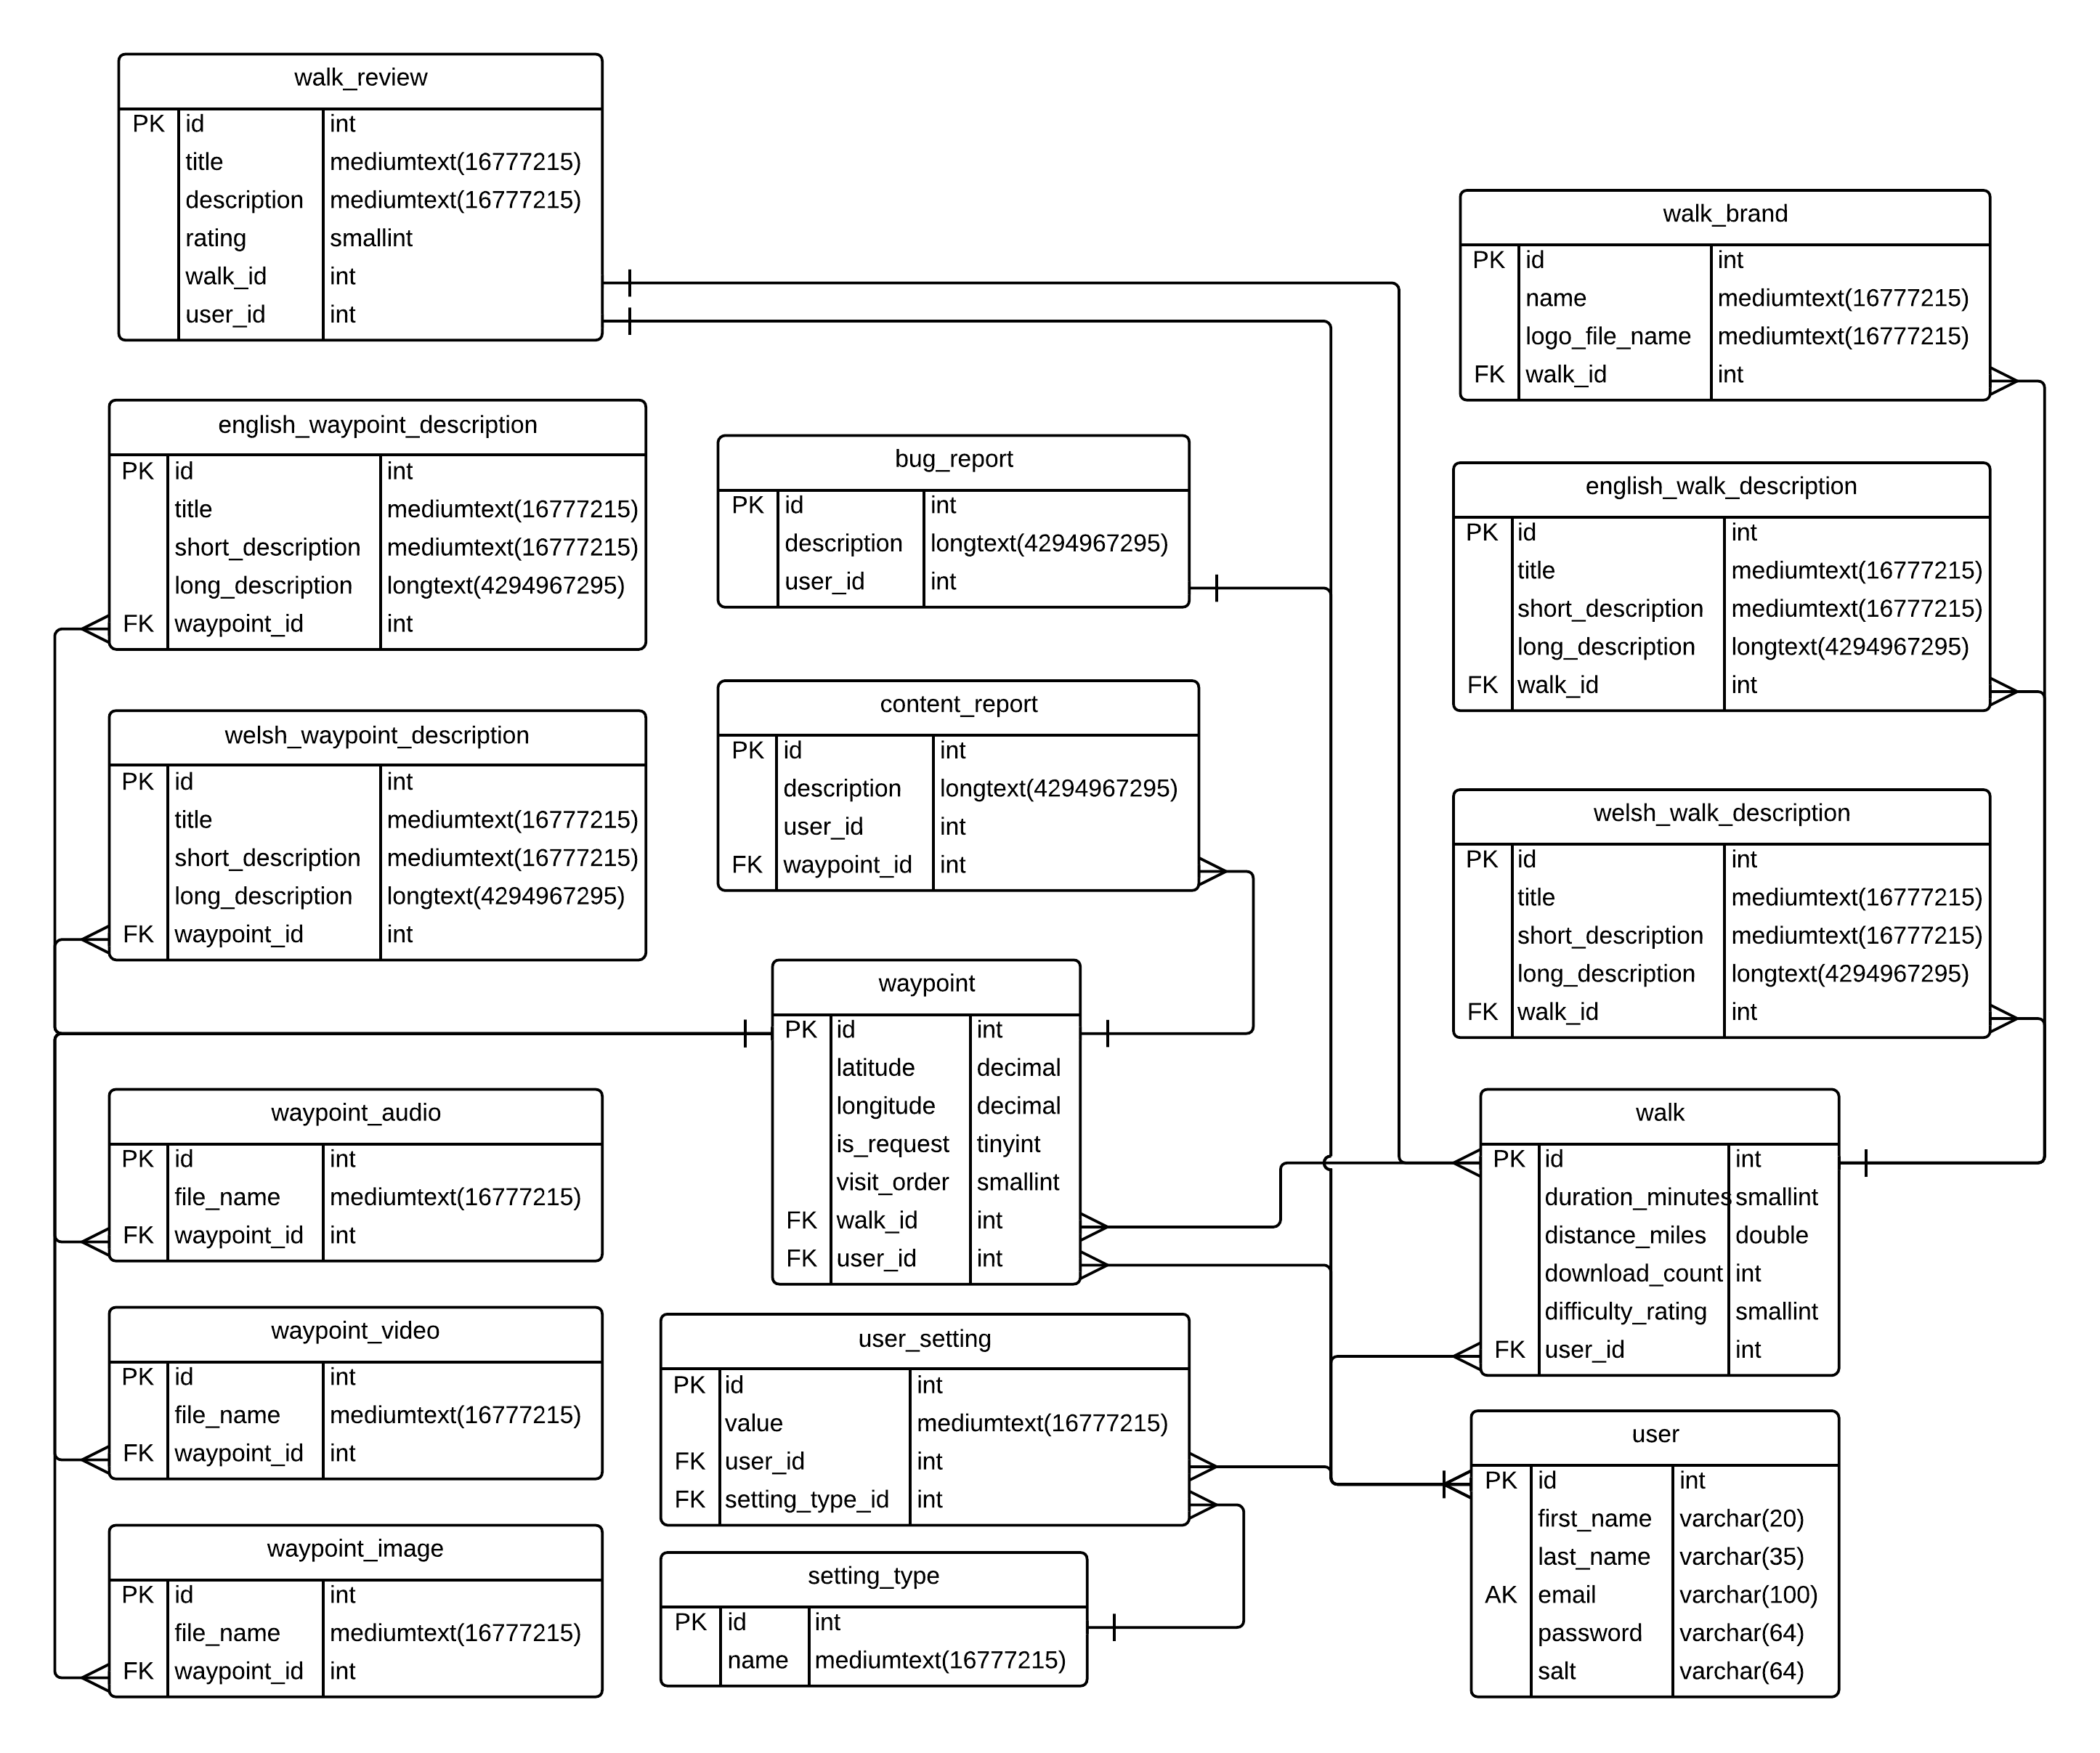
\includegraphics[angle=90, width=1\linewidth]{./img/DatabaseSchema}
\caption{Schema of the White Rock Trails relational database.}
\label{fig:DatabaseSchema}
\end{figure}


\section{User Interface Design}
%- Heuristic Evaluations on similar products
%-- Explain how we are doing the evaluation blahblah nielsen etc.
%-- List of tasks for evaluators to complete (we should really ALL be involved in doing the evaluations).
%-- Problems found when completing each task
%- Our prototype UI 1
%-- show how it meets reqs, how heuristics helped design.
%-- Heuristics on this etc.
%- Our prototype UI 2
%-- show it meets reqs, how heuristics helped design.
%-- Heuristics
%- repeat as necessary.

\section{Android Application Progress}
\lstset{language=Java,
keywordstyle=\color{Maroon},
commentstyle=\color{OliveGreen},
showstringspaces=false, tabsize=4, breaklines=true, showspaces=false, stringstyle=\color{Blue}}
The development of the Android application is progressing well and has been unaffected by risks, both expected and unexpected. To achieve the goals of the project, the application has to be capable of saving and loading data to and from a local database, which will then synchronise with the remote database - this is achieved via a ContentProvider, seen in Section~\ref{sec:contentprovier}; the client also requested Google Maps be implemented, the progress of which can be seen in Section~\ref{sec:googlemaps}; as the application allows users to log-in and personalise their experience an authentication system has been created, seen in Section~\ref{sec:authorisation}. Finally, fragments and activities have been created to control the flow of the program, along with relevant layouts and graphics, which can be seen in Section~\ref{sec:fragments}. All of these systems, when completed, will meet the requirements shown in Section 4.1.2 of the Milestone 1 document. %TODO: Cite
\subsection{ContentProvider}
\label{sec:contentprovier}
The ContentProvider provides valuable functionality when synchronising with the server and allowing for other applications to, potentially, access the application's database. It consists of four components. Firstly, there is the DbSchema class, this interface class contains all of the SQL used to create the table and constants such as table names. Next comes the DatabaseHandler class, an extension of the Android SQLiteOpenHelper class, which creates the database and contains the strategy for deleting and upgrading the database; it is also responsible for opening and closing connections to the database. The WhiteRockContract class provides an API for foreign applications to access available data, without this the ContentProvider does not achieve anything. Finally, there is the WhiteRockContentProvider class itself, this class is responsible for inserting, deleting, updating and querying the database.

\subsubsection{Database Schema}
The DbSchema class is an interface which is strictly used for referencing constants, such as table names, and strings containing the SQL used to create each table in the database. Example code can be seen in Listing~\ref{lst:dbSchema}.

\begin{lstlisting}[captionpos=b, caption=DbSchema Snippet, label=lst:dbSchema, frame=single]
	// Example code snippet from DbSchema.java
	
	String VIEW_WAYPOINT_WITH_ENGLISH_DESCR = "waypoint_and_english";
	
	String CREATE_TABLE_WALK = 
			"CREATE TABLE `walk` (" 
			+"_id INTEGER PRIMARY KEY AUTOINCREMENT ,"
			+"duration_minutes INT,"
			+"distance_miles REAL,"
			+"download_count INT,"
			+"difficulty_rating INT,"
			+"user_id INT"
			+")";
	
	String CREATE_TABLE_WALK_BRAND = 
			"CREATE TABLE `walk_brand` ("
			+"_id INTEGER PRIMARY KEY AUTOINCREMENT ,"
			+"name TEXT,"
			+"logo_file_name TEXT,"
			+"walk_id INT"
			+")";
			
\end{lstlisting}

\subsubsection{DatabaseHandler}
Responsible for creating, deleting and upgrading the database, as well as opening and closing connections, the DatabaseHandler class is vital for both maintaining the database and interfacing with it.

Listing~\ref{lst:dbHandler} provides a snippet of the code used during the creation of a DatabaseHandler instance and how it uses the DbSchema to create the database.

\begin{lstlisting}[captionpos=b, caption=DatabaseHandler Snippet, label=lst:dbHandler, frame=single]
	public DatabaseHandler(Context context) {
		super(context, DB_NAME, null, DB_VERSION);
		
		// Find the correct path based on Android version.
		if (android.os.Build.VERSION.SDK_INT >= Build.VERSION_CODES.JELLY_BEAN_MR1) {
			DB_PATH = context.getApplicationInfo().dataDir + "/databases/";
		} else {
			DB_PATH = "/data/data/" + context.getPackageName() + "/databases/";
		}
		Log.d(TAG,"DB Path is: " + DB_PATH+DB_NAME);
		Log.d(TAG, "Version Number: " + android.os.Build.VERSION.SDK_INT);
		this.mContext = context;
	}

	@Override
	public void onCreate(SQLiteDatabase db) {
		Log.d(TAG, "CREATING");
		// create User tables
		db.execSQL(DbSchema.CREATE_TABLE_USER);
		db.execSQL(DbSchema.CREATE_TABLE_SETTING_TYPE);
		db.execSQL(DbSchema.CREATE_TABLE_USER_SETTINGS);
		
		// Create Walk Tables
		db.execSQL(DbSchema.CREATE_TABLE_WALK);
		db.execSQL(DbSchema.CREATE_TABLE_WALK_BRAND);
		db.execSQL(DbSchema.CREATE_TABLE_WALK_REVIEW);
		db.execSQL(DbSchema.CREATE_TABLE_ENGLISH_WALK_DESCR);
		db.execSQL(DbSchema.CREATE_TABLE_WELSH_WALK_DESCR);
	}
\end{lstlisting}

\subsubsection{WhiteRockContract}
The WhiteRockContract class is the API which all applications, including this one, must use to access the ContentProvider. The class itself is relatively simple, providing constant values for the Authority and Content URI's required to access the data. The ContentProvider accesses data from the database by being passed a URI in the format content://authority//path\_to\_type. In this implementation the authority is ``uk.ac.swan.digitaltrails'' the path\_to\_type variable points to a table name, such as ``walk''. An example of this, for the ``bug\_report'' table, can be seen in Listing~\ref{lst:contract}.

\begin{lstlisting}[captionpos=b, caption=WhiteRockContract Snippet, label=lst:contract, frame=single]
public class WhiteRockContract {
	
	public static final String AUTHORITY = "uk.ac.swan.digitaltrails";
	public static final Uri CONTENT_URI = Uri.parse("content://" + AUTHORITY);


	/**
	 * Constants for Bug Report table.
	 * @author Lewis Hancock
	 *
	 */
	public static final class BugReport implements ReportColumns {
		public static final Uri CONTENT_URI = Uri.withAppendedPath(
				WhiteRockContract.CONTENT_URI, "bug_report");
	
		public static final String CONTENT_TYPE = ContentResolver.CURSOR_DIR_BASE_TYPE +
				"vnd.uk.ac.swan.digitaltrails.bug_report";
		
		public static final String CONTENT_TYPE_DIR = ContentResolver.CURSOR_ITEM_BASE_TYPE +
				"vnd.uk.ac.swan.digitaltrails.bug_report";
		
		public static final String SORT_ORDER_DEFAULT = ID + " ASC";
		
		public static final String[] PROJECTION_ALL = {ID, DESCRIPTION, USER_ID};

	}
	// rest of code omitted
}
\end{lstlisting}


\subsubsection{WhiteRockContentProvider}
The WhiteRockContentProvider class is where all of the components come together. A URIMatcher is created to ensure that the correct data is accessed, according to the content URI passed. Based on the call to the ContentProvider (insert, update, delete, query), the URI passed is matched via the URIMatcher and the operation carried out on the correct data in the correct table. Examples of each operation can be seen in Listing~\ref{lst:contentprovider}.

\begin{lstlisting}[captionpos=b, caption=WhiteRockContentProvider Snippet, label=lst:contentprovider, frame=single]
	private static UriMatcher buildUriMatcher() {
		final UriMatcher matcher = new UriMatcher(UriMatcher.NO_MATCH);
		final String authority = WhiteRockContract.AUTHORITY;
		matcher.addURI(authority, "walk", WALK_LIST);
		matcher.addURI(authority, "walk/#", WALK_ID);
		matcher.addURI(authority, "english_walk_description", ENGLISH_WALK_DESCR_LIST);
		matcher.addURI(authority, "english_walk_description/#", ENGLISH_WALK_DESCR_ID);
		matcher.addURI(authority, "welsh_walk_description", WELSH_WALK_DESCR_LIST);
		matcher.addURI(authority, "welsh_walk_description/#", WELSH_WALK_DESCR_ID);
	}
	
		@Override
		public boolean onCreate() {
			Context context = getContext();
			mDbHandler = new DatabaseHandler(context);
			return true;
		}
		
		@Override
		public int delete(Uri uri, String selection, String[] selectionArgs) {
			SQLiteDatabase db = mDbHandler.getWritableDatabase();
			int deleteCount = 0;
			String idStr;
			String where;
			
			switch (URI_MATCHER.match(uri)) {
			case WALK_LIST:
				deleteCount = db.delete(DbSchema.TABLE_WALK, selection, selectionArgs);
				break;
			case WALK_ID:
				idStr = uri.getLastPathSegment();
				where = WhiteRockContract.Walk._ID + " = " + idStr;
				if (!TextUtils.isEmpty(selection)) {
					where += " AND " + selection;
				}
				deleteCount = db.delete(DbSchema.TABLE_WALK, where, selectionArgs);
				break;
				// Rest of code omitted.
			}
			return deleteCount;
		}
		
		@Override
		public Uri insert(Uri uri, ContentValues values) {
			SQLiteDatabase db = mDbHandler.getWritableDatabase();
			long id = 0;
			switch (URI_MATCHER.match(uri)) {
			case WALK_LIST:
				id = db.insert(DbSchema.TABLE_WALK,
							  null,
						      values);
				db.close();
				return getUriForId(id, uri);
			case WAYPOINT_LIST:
				id = db.insert(DbSchema.TABLE_WAYPOINT,
							  null,
							  values);
				db.close();
				Log.d(TAG, "Attempting insert into waypoint table");
				return getUriForId(id, uri);
				
				// Rest of code omitted
			}
		}
		
		@Override
		public Cursor query(Uri uri, String[] projection, String selection, String[] selectionArgs,
				String sortOrder) {
			SQLiteDatabase db = mDbHandler.getReadableDatabase();
			SQLiteQueryBuilder builder = new SQLiteQueryBuilder();
			String queryString;
			boolean useAuthorityUri = false;
			switch (URI_MATCHER.match(uri)) {
			case WALK_LIST:
				builder.setTables(DbSchema.TABLE_WALK);
				if (TextUtils.isEmpty(sortOrder)) {
					sortOrder = WhiteRockContract.Walk.SORT_ORDER_DEFAULT;
				}
				break;
			case WALK_ID:
				builder.setTables(DbSchema.TABLE_WALK);
				builder.appendWhere(WhiteRockContract.Walk._ID + " = " + uri.getLastPathSegment());
				break;
				// rest of code omitted
			}
			Log.d(TAG, builder.getTables());
			Cursor cursor = builder.query(db, projection, selection, selectionArgs, null, null, sortOrder);
			if (useAuthorityUri) {
				cursor.setNotificationUri(getContext().getContentResolver(), WhiteRockContract.CONTENT_URI);
			} else {
				cursor.setNotificationUri(getContext().getContentResolver(), uri);
			}
			return cursor;
		}
		
		@Override
		public int update(Uri uri, ContentValues values, String selection, String[] selectionArgs) {
	
			SQLiteDatabase db = mDbHandler.getWritableDatabase();
			int updateCount = 0;
			String idStr;
			String where;
	
			switch(URI_MATCHER.match(uri)) {
			case WALK_LIST:
				updateCount = db.update(DbSchema.TABLE_WALK, values, selection, selectionArgs);
				break;
			case WALK_ID:
				idStr = uri.getLastPathSegment();
				where = WhiteRockContract.Walk._ID + " = " + idStr;
				if (!TextUtils.isEmpty(selection)) {
					where += " AND " + selection;
				}
				updateCount = db.update(DbSchema.TABLE_WALK, values, where, selectionArgs);
				break;
				// rest of code omitted.
			}
			return updateCount;
		}
	
\end{lstlisting}

\subsubsection{Using the ContentProvider}
The ContentProvider is currently being used, in conjunction with a CursorLoader, to query the database for walk names to choose a walk and, when a walk has been chosen, the waypoint details of that walk. The CursorLoader is an asynchronous loader, allowing data to be loaded in a different thread than the User Interface thread. This is great for loading the user interface whilst the data is loading. All the relevant code for loading data, in this example the titles of each walk and their details, can be seen in Listing~\ref{lst:walkListFragment}.

\begin{lstlisting}[captionpos=b, caption=WalkListFragment Snippet, label=lst:walkListFragment, frame=single]

public class WalkListFragment extends ListFragment 
	implements LoaderCallbacks<Cursor>, OnQueryTextListener {

	// Non-relevant code omitted.

	static String [] WALK_SUMMARY_PROJECTION = {WhiteRockContract.EnglishWalkDescriptions._ID, WhiteRockContract.EnglishWalkDescriptions.TITLE, WhiteRockContract.EnglishWalkDescriptions.WALK_ID };
	
	@Override
	public void onActivityCreated(Bundle savedInstanceState) {
		super.onActivityCreated(savedInstanceState);
		
		//setHasOptionsMenu(true);
		setEmptyText("No Walks");	//TODO load this from resource.
		mAdapter = new SimpleCursorAdapter(getActivity(), mLayout, null,
					new String[] {WhiteRockContract.EnglishWalkDescriptions.TITLE },
					new int[] {android.R.id.text1}, 0);	
		setListAdapter(mAdapter);
		setListShown(false);
		// Load the data!
		getLoaderManager().initLoader(0, null, this);
	}

	
	@Override
	public Loader<Cursor> onCreateLoader(int id, Bundle args) {
		Uri baseUri;
		if (mCurFilter != null) {
			baseUri = Uri.withAppendedPath(WhiteRockContract.CONTENT_URI, Uri.encode(mCurFilter));
		} else {
			baseUri = WhiteRockContract.EnglishWalkDescriptions.CONTENT_URI;
		}
		
		String select = "((_id))";
		return new CursorLoader(getActivity(), baseUri, WALK_SUMMARY_PROJECTION, select, null, WhiteRockContract.EnglishWalkDescriptions.WALK_ID + " COLLATE LOCALIZED ASC");
	}

	@Override
	public void onLoadFinished(Loader<Cursor> loader, Cursor data) {
		mAdapter.swapCursor(data);
		
		if (isResumed()) {
			setListShown(true);
		} else {
			setListShownNoAnimation(true);
		}
		
	}

	@Override
	public void onLoaderReset(Loader<Cursor> arg0) {
		mAdapter.swapCursor(null);
	}
}
\end{lstlisting}

All of the code (and more) in the above sections results in the screens and interactions seen in Figures~\ref{fig:walkListFragment} and~\ref{fig:googleContentLoader} being available in the application at the time of writing. This code is now completed, unless it becomes clear that we need access to other areas of the database.

\begin{figure}[H]
\centering
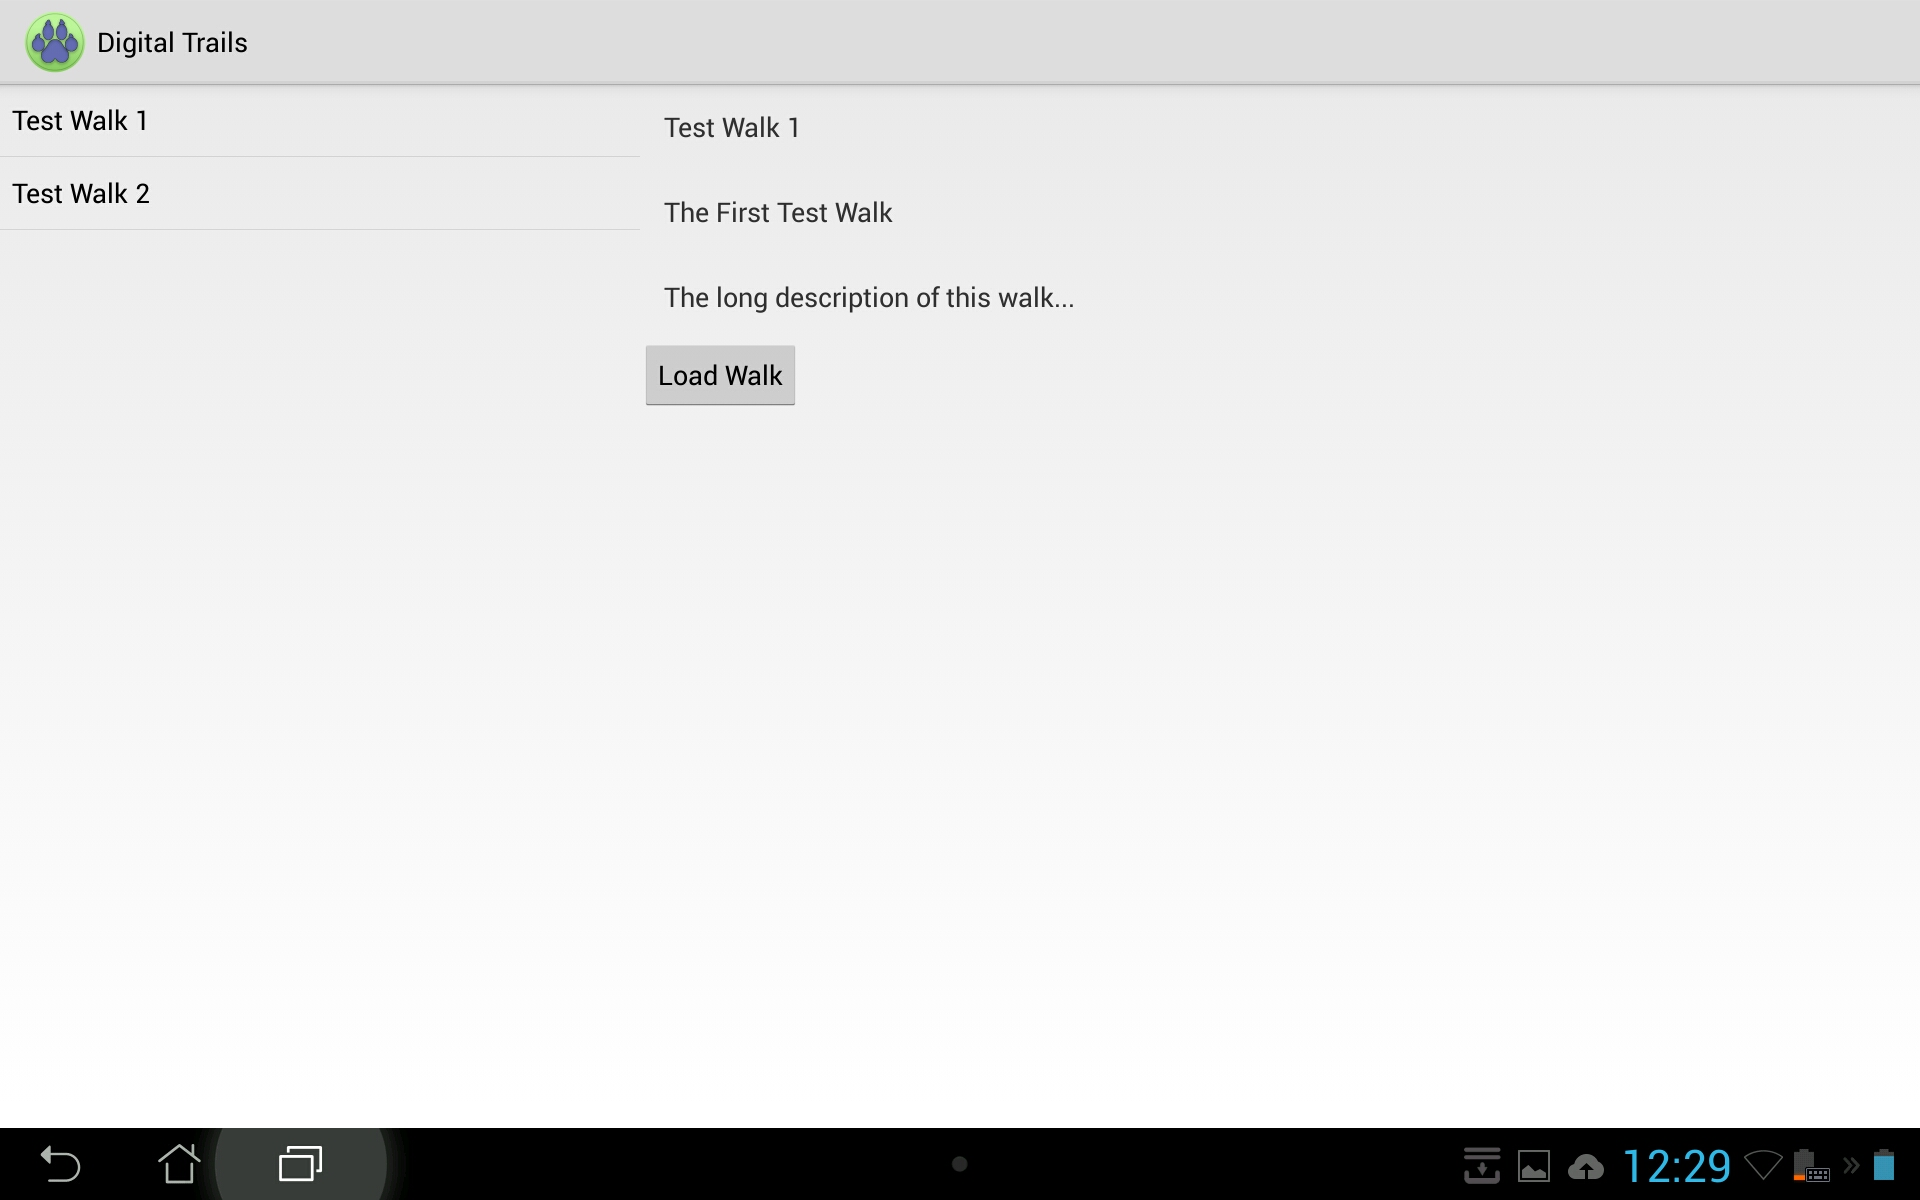
\includegraphics[angle=90, width=.5\linewidth]{walkListFragment.jpg}
\caption{Screenshot of WalkListFragment Fragment loading walk details from the database.}
\label{fig:walkListFragment}
\end{figure}


\begin{figure}[H]
\centering
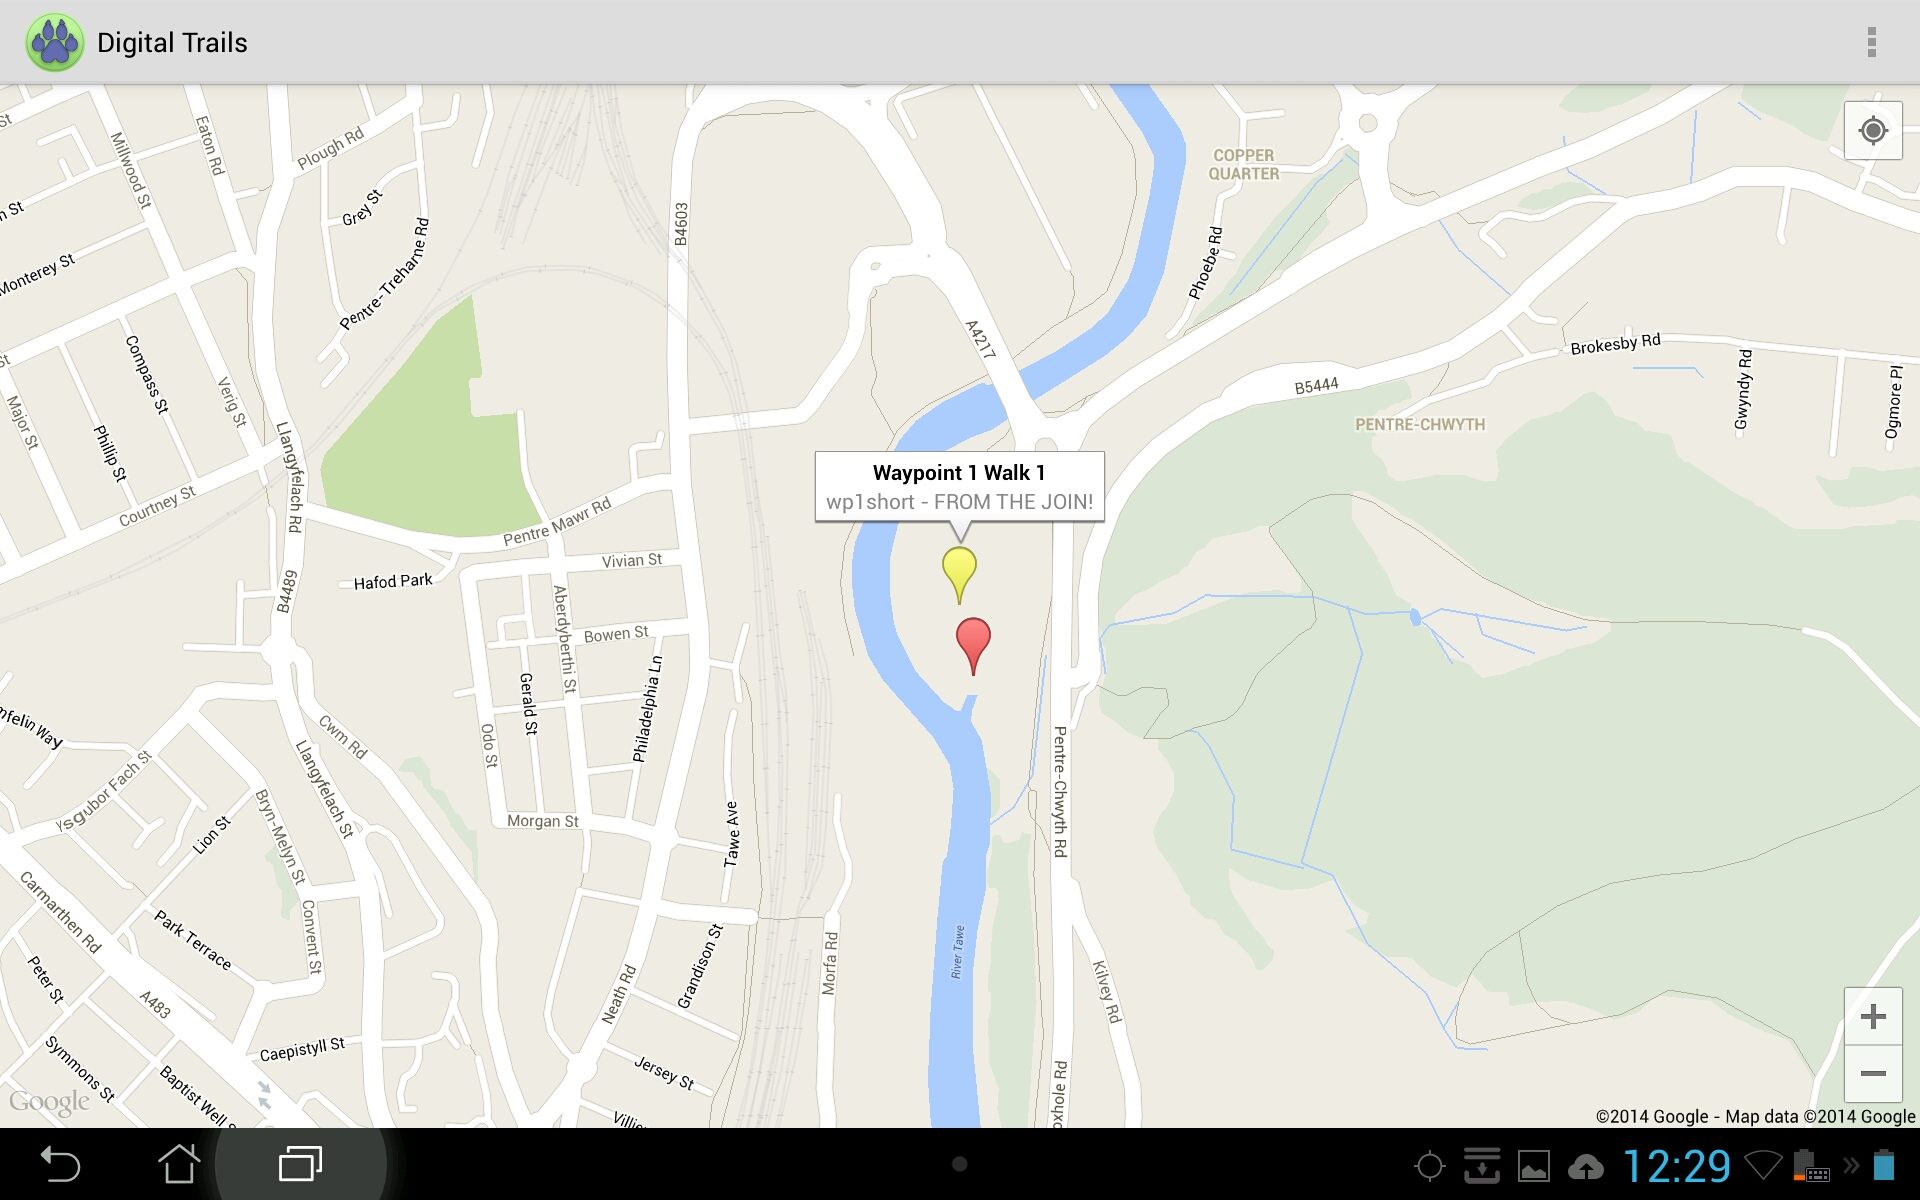
\includegraphics[angle=90, width=.6\linewidth]{googleMapsContentLoader.jpg}
\caption{Screenshot of the MapActivity displaying waypoint details from the database.}
\label{fig:googleContentLoader}
\end{figure}


\subsection{Google Maps}
\label{sec:googlemaps}
Currently the Google Maps API has been integrated at a basic level. The user can select a walk and the correct data will be displayed on the Map, with tappable waypoint markers. After tapping a marker a small information area (InfoWindow) will appear, this gives the waypoint title and the short description of it. Tapping on this area will display a large dialog, displaying all the information available for that waypoint. These interactions can be seen in Figures~\ref{fig:googleContentLoader} and~\ref{fig:wpInfoDialog}.

\begin{figure}[H]
\centering
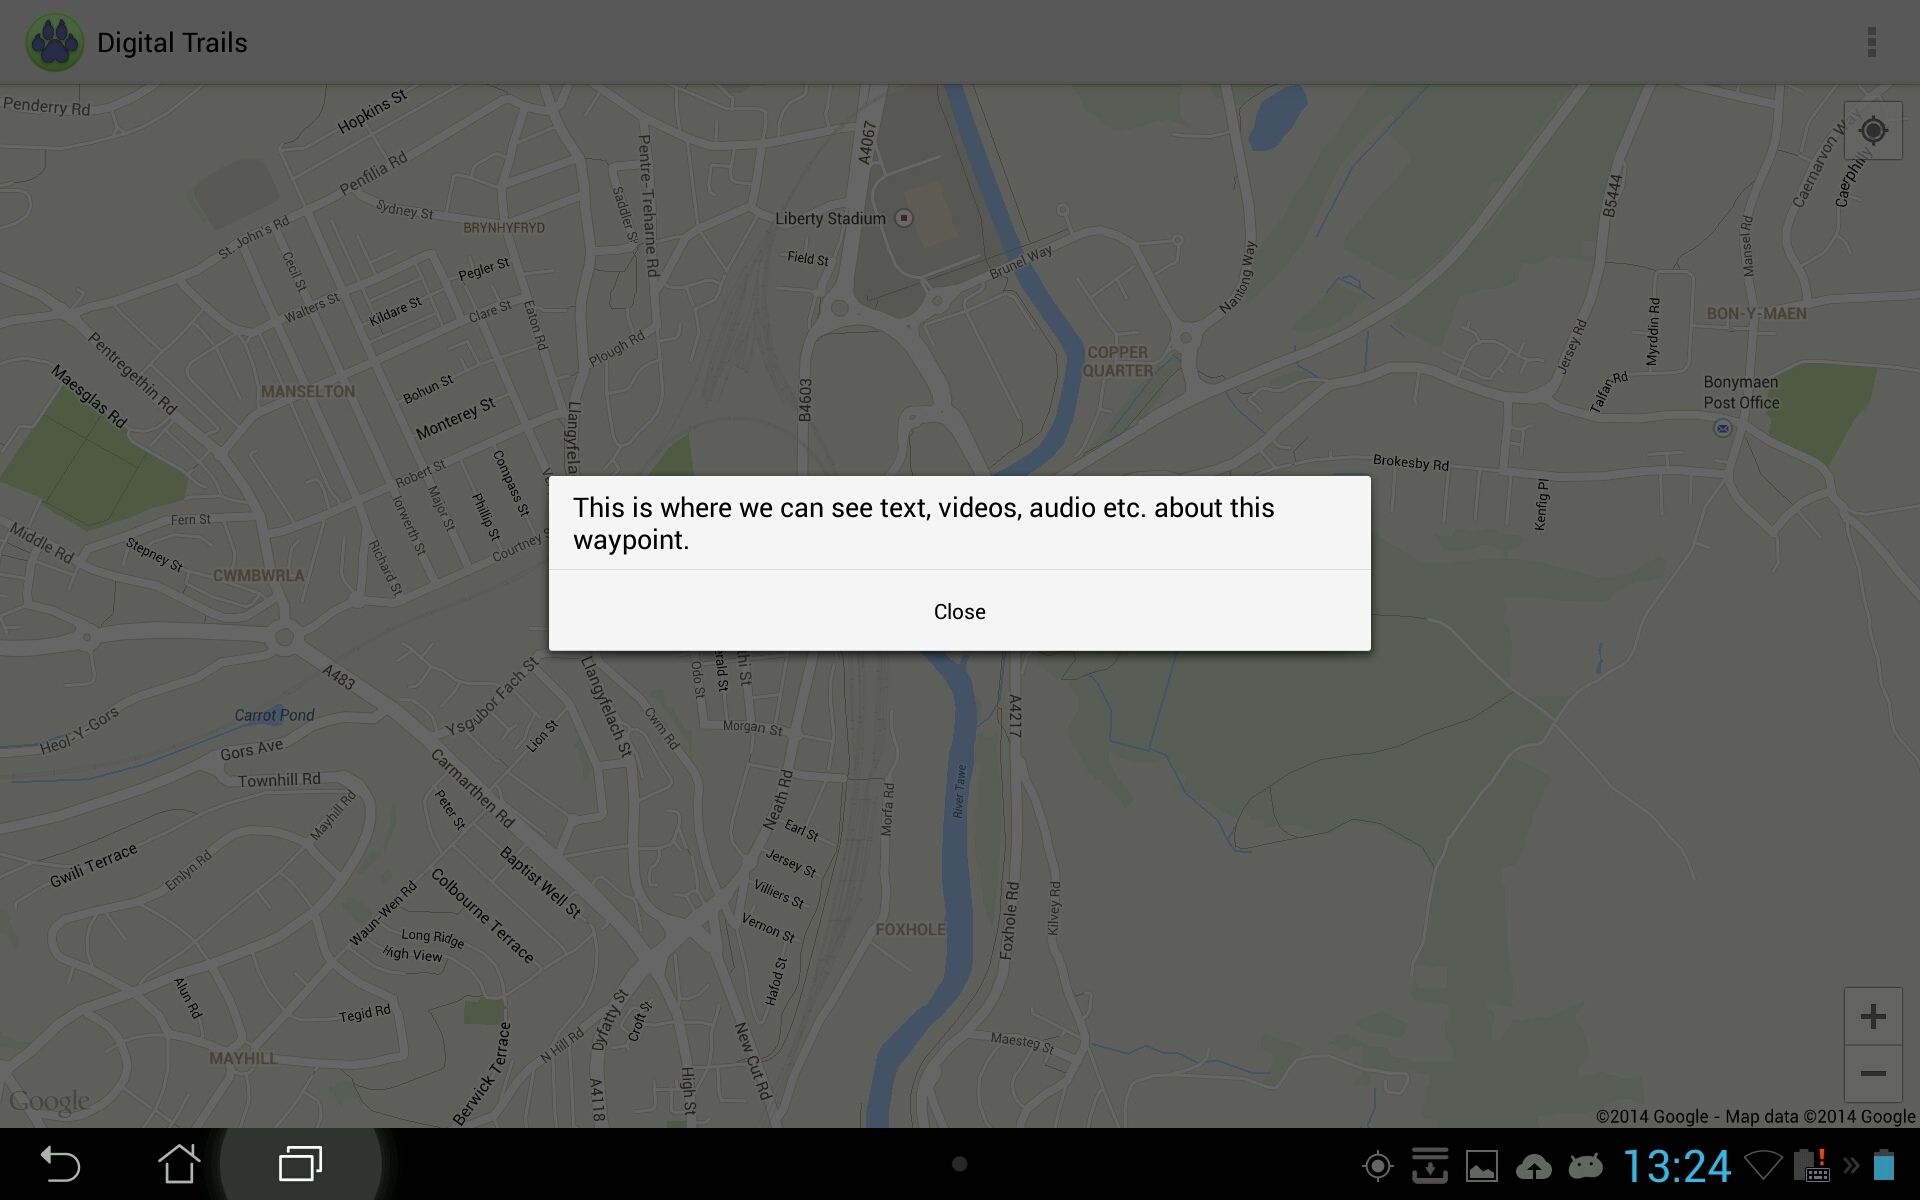
\includegraphics[angle=90, width=.6\linewidth]{wpInfoDialog.jpg}
\caption{Screenshot of the MapActivity Information Dialog.}
\label{fig:wpInfoDialog}
\end{figure}

Users may also change the style of the map to ``Normal'', ``Hybrid'' or ``Satellite''; rotate, zoom, pan and tilt the map with gestures and zoom the map in and out and find the user's current location with on-screen buttons. These can be see in Figures~\ref{fig:mapOptions} and~\ref{fig:userLocation}.

\begin{figure}[H]
\centering
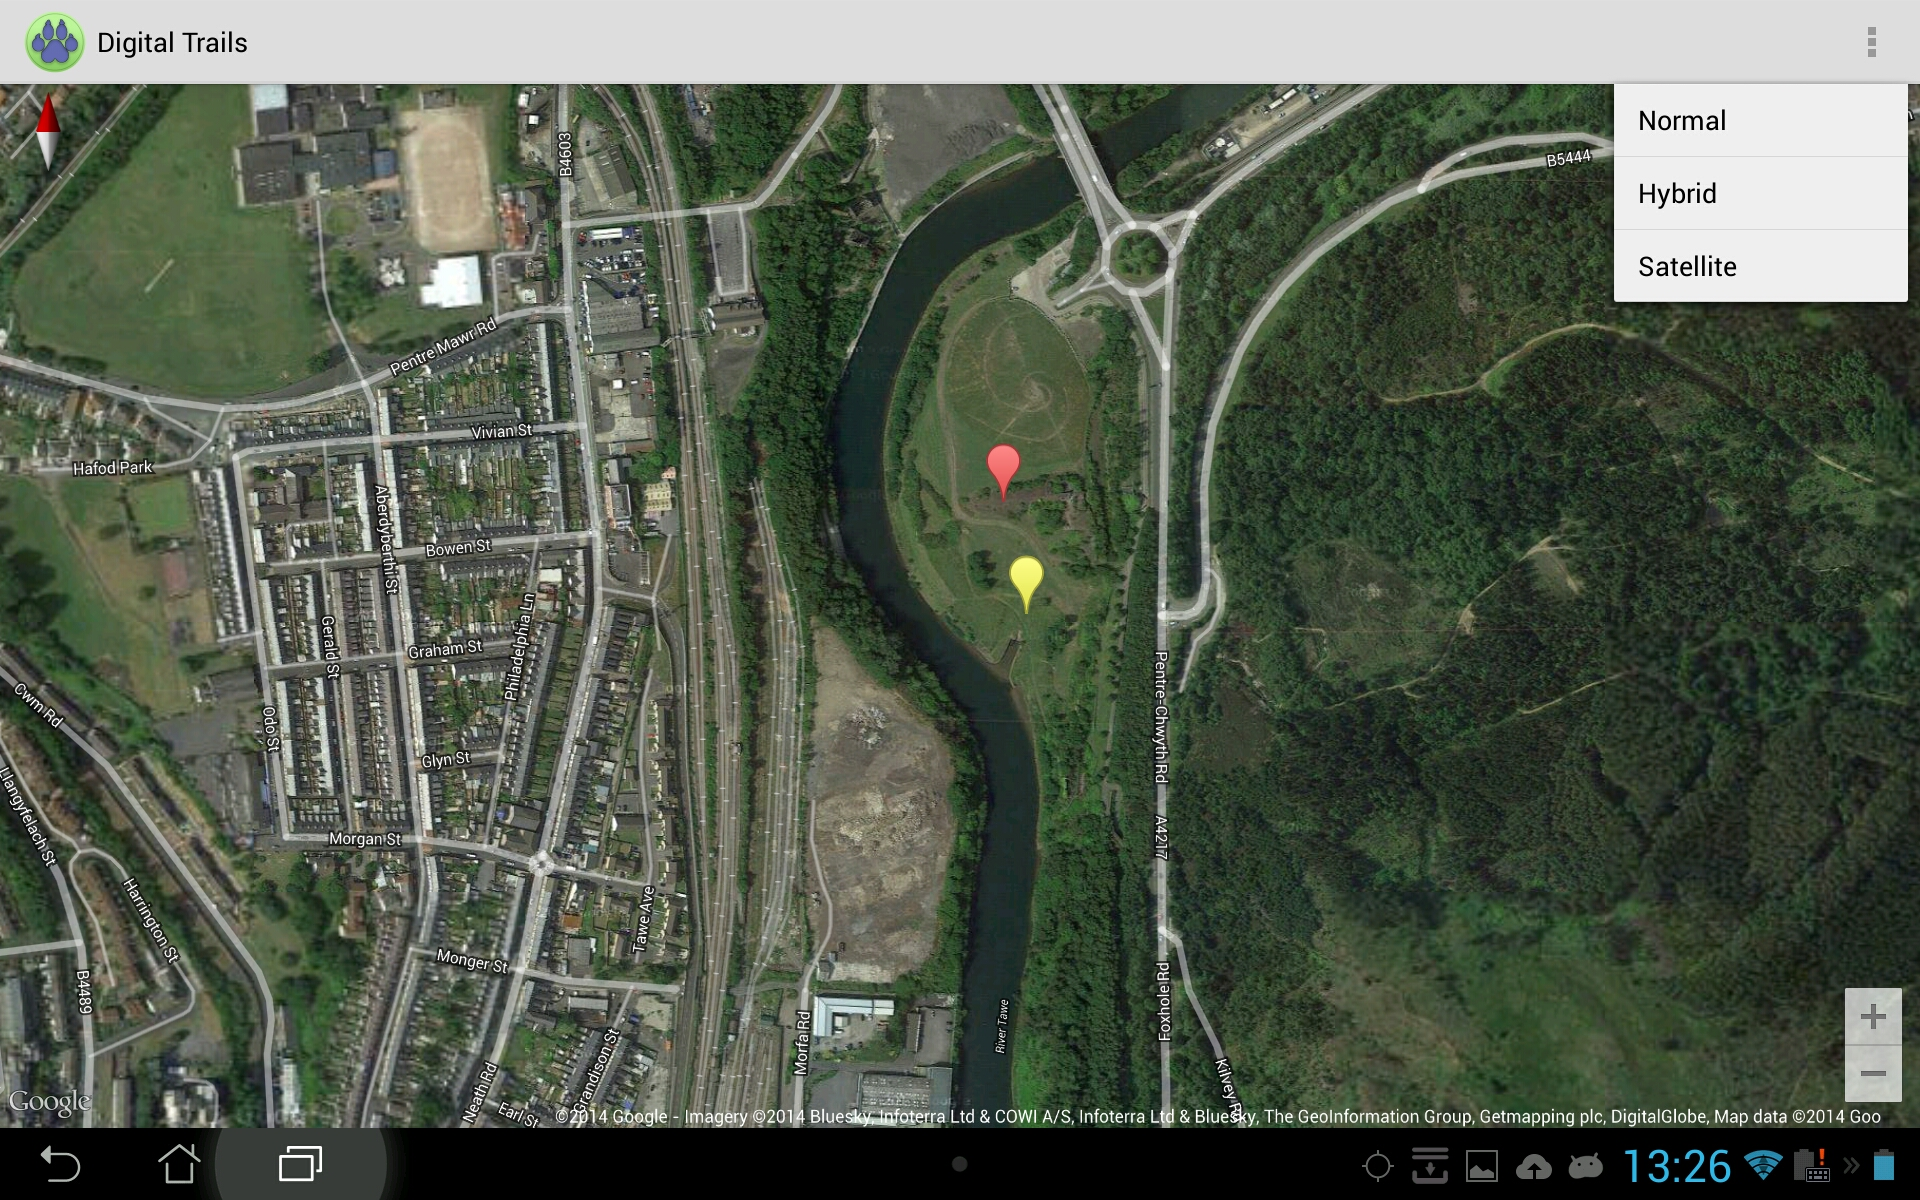
\includegraphics[angle=90, width=.6\linewidth]{mapOptions.jpg}
\caption{Screenshot of the MapActivity map options.}
\label{fig:mapOptions}
\end{figure}

\begin{figure}[H]
\centering
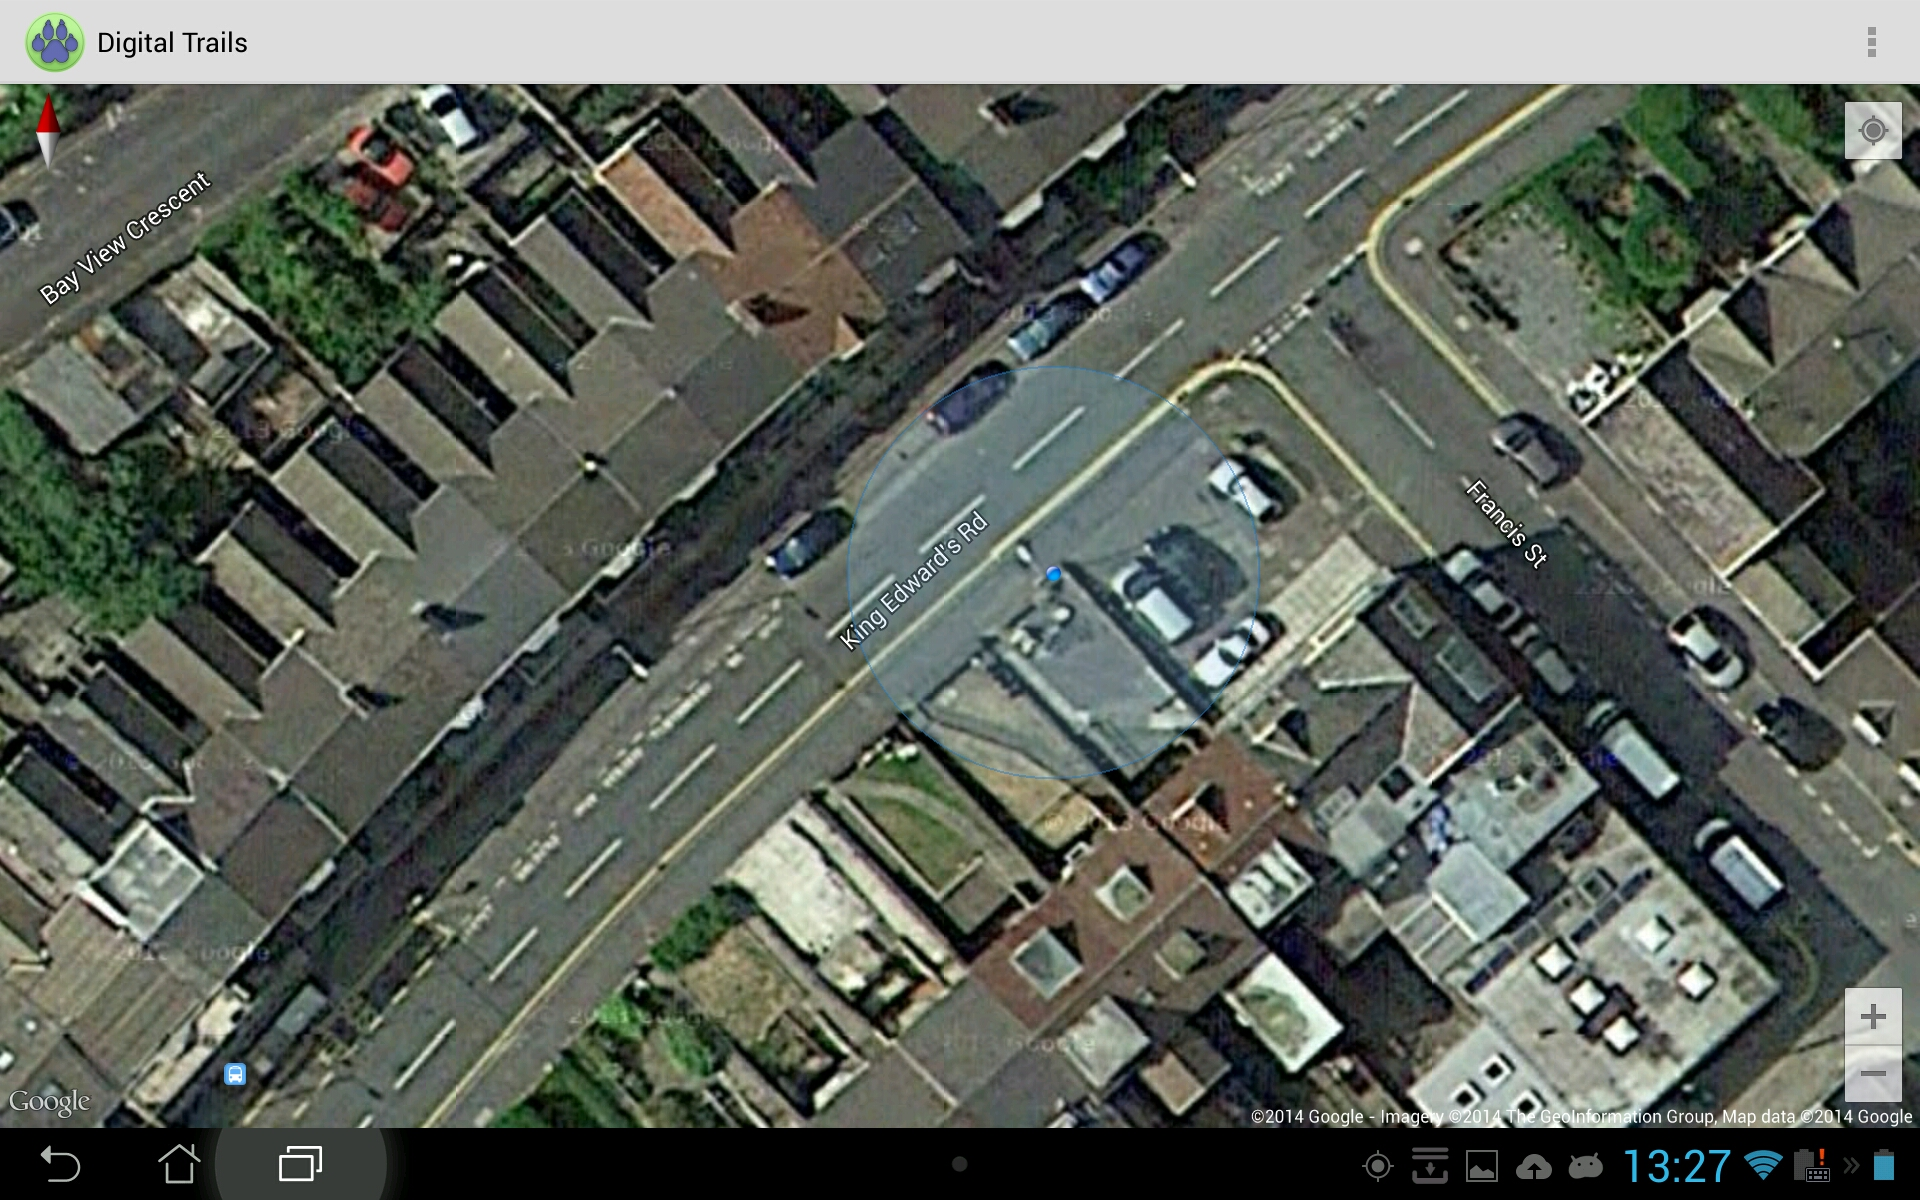
\includegraphics[angle=90, width=.6\linewidth]{userLocation.jpg}
\caption{Screenshot of the MapActivity displaying user's current location.}
\label{fig:userLocation}
\end{figure}

Future development includes creating a custom InfoWindowAdapter for the InfoWindow, allowing for more customisable data to be displayed. The next waypoint to visit shall be displayed in a different colour than the other waypoints, whilst previously visited waypoints will also change colour. 


\subsection{Authentication}
\label{sec:authorisation}

\subsection{Fragments}
\label{sec:fragments}

\subsection{SyncAdapter}
\label{sec:syncAdapter}
Whilst not currently implemented, the ContentProvider and Authentication systems are a vital part of this system and it is the foremost reason the ContentProvider was created. The SyncAdapter handles background synchronisation of data from the Android application to the tablet and vice-versa. It is triggered when needed, scheduled or requested. It is the preferred system compared to using Services and IntentServices as it provides an implementation which is:
\begin{itemize}
\item \textbf{Battery Efficient} By being scheduled to run when other synchronisations run, the application is conserving battery power by leaving the device sleeping for as long as possible.
\item \textbf{User Friendly} The SyncAdapter may be accessed by the user from the Android Settings screen, allowing for customisation of the SyncAdapter's settings and even the ability to disable it.
\item \textbf{Content Aware} The ContentProvider which has been written will allow the SyncAdapter to monitor the data and only synchronise with the remote server when the data has been updated.
\item \textbf{Capable of Retrying} The implementation of a SyncAdapter provides it with a retry mechanism, allowing for data to be synchronised as soon as possible.
\end{itemize}

Further information can be found at \url{http://developer.android.com/training/sync-adapters/index.html}.


\subsection{API}

A RESTful API has been created using the technologies discused in section \ref{sec:techAPI}. There are several important parts to the API, first it must have a coherent set of routes/urls for acces to all if its functionality, secondly it must provide a method of authenticating users and finaly it must adhear to to principles of REST as closely as possible. 

\subsubsection{Routes}

The API is called through a series of routes, it was important to make these routes as simple and coherant as possible.

\begin{longtable}{m{0.45\textwidth}|m{0.35\textwidth}|C{0.11\textwidth}}\hline
    \textbf{Route} & \textbf{Return value} & \textbf{Methods} \\\hline
    /walks & All walks & GET POST\\ \hline
    /walks/\$id & The walks with the ID \$id. & GET PUT DELETE\\ \hline
    /walks/\$id/waypoints & All the waypoints for the walk with the ID \$id. & GET POST\\ \hline
    /walks/\$id/waypoints/\$wid & The waypoint with the ID \$wid. & GET PUT DELETE \\ \hline
    /walks/\$id/waypoints/\$wid/images & The images for the waypoint with the ID \$wid. & GET POST \\ \hline
    /walks/\$id/waypoints/\$wid/images/\$iid & The image with the ID \$iid. & GET PUT DELETE \\ \hline
    /walks/\$id/waypoints/\$wid/audio & The audio files for the waypoint with the ID \$wid. & GET POST \\ \hline
    /walks/\$id/waypoints/\$wid/audio/\$aid & The audio file with the ID \$aid. & GET PUT DELETE \\ \hline
    /walks/\$id/waypoints/\$wid/videos & The videos for the waypoint with the ID \$wid. & GET POST \\ \hline
    /walks/\$id/waypoints/\$wid/videos/\$vid & The video with the ID \$vid. & GET PUT DELETE \\ \hline
    /users & All users. & GET POST \\\hline
    /users/\$id & The user with the ID \$id. & GET PUT DELETE \\\hline
    /users/\$id/settings & A users settings. & GET PUT \\\hline
    /session & A request to authenticate. & GET\\\hline
    /session/salt & Returns a random salt for registering a user. & GET\\\hline
    /session/salt/\$username & Get the a salt for a specific user with the username \$username. & GET\\\hline
    \caption {The routes for the API}
    \label{routes}
\end{longtable}

The routes are structured in such a way that they help the user find the data they are looking for. They are structured similar to the database structure with waypoints belonging to walks and images, audio and videos belonging to waypoints. 

To reduce load on the server any request will also return all the data that belongs to it, this means when a walk is requested it will contain all of its waypoints along with the media for each waypoint. This ensures the server is not overloaded with requests and will increase the speed of applications using the API as fewer requests are required. 


\subsection{Web Portal}

\subsubsection{Web Application}

\section{Coding Guidelines}
A set of coding guidelines have been created for both the Android and Web applications. This will ensure that developers can quickly adapt to and understand the code of team members, reducing unnecessary downtime and interruptions. The main rule of the guidelines is to practice a consistent coding style, which is to say that code which a developer writes should be consistent with other code that is being modified as well as consistent when looked at alone.
\subsection{Android}
TODO: Say adapted from Lewis' document.
\begin{itemize}
\item \textbf{Declaring Variables}
	\begin{enumerate}
	\item All non-static, non-public member variables begin with a lower case m (e.g. mMyVariable).
	\item All static variables begin with a lower case s (e.g. sStaticClass).
	\item All class member variables are private.
	\item Variable names begin with a lower case letter, then each consecutive word in the variable's name begins with an upper-case letter.
	\item Each variable will be declared on a separate line.
	\item A variable should be declared only when needed.
	\item Variable names should be as descriptive as possible, avoid unnecessary abbreviations.
	\item Classes always begin with an upper-case letter.
	\item File names always match class names.
	\item Constant variables are defined in upper-case, with an underscore between words.
	\end{enumerate}
\item \textbf{Whitespace}
	\begin{enumerate}
	\item Always use a single space after a keyword and before a curly brace.
	\end{enumerate}
\item \textbf{Braces}
	\begin{enumerate}
	\item The opening brace goes on the same line as the statement, as is traditional in Java.
	\item Always use curly braces for conditional statements, even if it only contains one line.
	\end{enumerate}
\item \textbf{Documentation}
	\begin{enumerate}
	\item All methods and variables are to be documented with Doxygen, using standard Javadoc style comments.
	\end{enumerate}
\end{itemize}

%- Adam/Tom get on the web guidelines.

\section{Risk Analysis Review}
The project has encountered a selection of the risks outlined in the initial document. These risks are:
\begin{itemize}
\item\textbf{TECRSK2} Personal computers used for software development fail. This has occurred to Adam Barrell on at least one occasion. Thomas Milner has also had his server break, requiring it to be fully reconfigured. This cost us a day of development on the authentication system.
\item\textbf{TECRSK1} Tesco Hudl fails. The Hudl has began to experience a fault which causes part of the screen to become unresponsive to user input.
\item\textbf{TECRSK7} The Google Android API is too limited. This is true of the Google Maps API, it does not let the developer extend the Marker class, which would make development easier, nor does it allow for caching of map data for offline use, preventing a serious issue for trails which are in a location that does not receive a mobile data connection. There is, currently, a potential solution which lets us store cached data for a short period of time.
\end{itemize}
The team has also encountered unforeseen risks, detailed below:
\begin{itemize}
\item\textbf{Hudl Support} The Hudl is not seen as a developer device by Tesco, as a result they do not provide a USB driver. A workaround was discovered by forcing the development machine to install the generic Google USB driver to the device.
\item\textbf{Work Environment} The Swansea University Project Lab has been in a contentious state since the beginning of this academic year, with some staff claiming it is a common room whilst other claim it is for group project work. This left developers without a peaceful place to work, as a group, whilst on campus. This has, hopefully, since been rectified after the status of the room was confirmed with members of staff as a room to be used as a working environment. 
\item\textbf{Bugs in Libraries} The validation library being used for the website (Bootstrap Validator (TODO:CITE)) contained a number of bugs, delaying development of the website by a number of days whilst a bug report was processed by the library developer.
\item\textbf{AJAX Cross Origin Resource Sharing} TODO: Tom, write about this.
\item\textbf{Git User Error} Whilst not a risk which has yet caused a fatal incident, there have been times where user error has caused a delay whilst the local and remote Git repositories are restored to a working state.
\item\textbf{Lab Computers Have Restrictive Permissions} As the lab computers are so restrictive, the development team has not been able to implement the previously mentioned workaround for the Hudl device on one of the Swansea University computers. This prevents developers from using these systems for development. It is also not possible to install new software as required, which includes libraries, thus further increasing the difficulty in which these machines can be used.
\item\textbf{Communication Between Server and Android} This feature has shown itself to require more time than initially expected, to be efficient in both battery and data usage a ContentProvider and SyncAdapter have to be implemented. This adds extra layers of abstraction between the database and the application.
\item\textbf{Initial Code} The initial code the team was given to build upon was not sufficient to continue development, all the data had been hard-coded and strongly died to the OpenStreetMaps implementation. After analysing, commenting and reviewing the code it was deemed faster to begin with a new codebase, capable of using a ContentProvider and SyncAdapter to handle data.
\end{itemize}

\section{Project Schedule Review}
%- What sprints we have completed.
%- What reqs / specifications are completed Chris Lewis' favourite job!).
%- Are we ahead or behind schedule? (hard for us to answer)
%- Did we have to modify any requirements / specs to get this far? Did we add any or drop any?
%- Create new gantt chart and compare it with the initial one.
%- Update online sprint software, make it look like we completed sprints on time.
%- Client feedback so far, previous client meetings, planned meetings, launch event we attended etc.

\section{Summary}
%- What we have planned next, I guess.

%References as subsection
\newpage
\bibliographystyle{plain}
\bibliography{bibliography}
\end{document}